\documentclass[11pt]{article}
\usepackage{amsmath, amsthm, epsfig, amsfonts, amssymb, listings, enumerate,
color, hyperref, mdframed}
\usepackage[utf8]{inputenc}
\usepackage[T1]{fontenc}
\usepackage{lmodern}
\usepackage[french]{babel}

\usepackage{fancyhdr}
\usepackage{lastpage}

\pagestyle{fancy}
\lhead{Programmation en C}
\chead{}
\rhead{EPFL -- Automne 2017}
\headsep = 24pt
\fancyfoot{}
\rfoot{\thepage\ / \pageref{LastPage}}
\renewcommand{\headrule}{\vbox to 0pt{\hbox to \headwidth{\dotfill}\vss}}
\fancyhfoffset[H]{0pt}
\renewcommand{\footrulewidth}{0pt}

\definecolor{dkgreen}{rgb}{0,0.6,0}
\definecolor{gray}{rgb}{0.5,0.5,0.5}
\definecolor{mauve}{rgb}{0.58,0,0.82}

\definecolor{mygray}{rgb}{0.4,0.4,0.4}
\definecolor{mygreen}{rgb}{0,0.8,0.6}
\definecolor{myorange}{rgb}{1.0,0.4,0}
\lstset{frame=tblr,
  language=[ANSI]C,
  aboveskip=3mm,
  belowskip=3mm,
  showstringspaces=false,
  columns=flexible,
  basicstyle={\small\ttfamily},
%  numbers=left,
  numberstyle=\tiny\color{gray},
  keywordstyle=\color{blue},
  commentstyle=\color{dkgreen},
  stringstyle=\color{mauve},
  breaklines=true,
  breakatwhitespace=true
  tabsize=3
}

\textheight 23cm
\textwidth 16.5cm
\voffset -2.5cm
\hoffset -2cm

\parindent 0cm
\parskip.5\baselineskip

\begin{document}

%========================
\begin{center}{\bf Session d'exercices -- Pointeurs}\\
\textbf{\emph{Moyenne glissante}}
\end{center}

En statistiques, une \textbf{moyenne glissante} (\textit{moving average} en anglais), consiste en la création d'une série de moyennes de différents sous-ensembles d'un ensemble de données.
En \textit{digital signal processing}, la moyenne glissante est souvent utilisée comme filtre sur un signal d'entrée.

Ci-dessous, nous avons deux exemples de calcul de moyenne glissante.
Pour chacun des exemples, la séquence d'entrée contient les dix éléments suivants (\textbf{échantillons}) 1, 2, 3, 4, 5, 5, 4, 3, 2, 1, ainsi que la taille du sous-ensemble utilisé pour la moyenne glissante \texttt{m = 3}.

\textbf{Example 1: Simple moving average}

La séquence de sortie (le résultat) est obtenue de la manière suivante: la moyenne du premier sous-ensemble est égale au premier échantillon de sortie ($average(1, 2, 3) = 2$).
La moyenne du sous-ensemble suivant est la valeur du second échantillon de sortie ($average(2, 3, 4) = 3$), etc.
La moyenne du dernier sous-ensemble est la valeur du dernier échantillon.
Cela a pour conséquence de produire une séquence de sortie qui contient deux éléments de moins que la séquence d'entrée.

\begin{center}
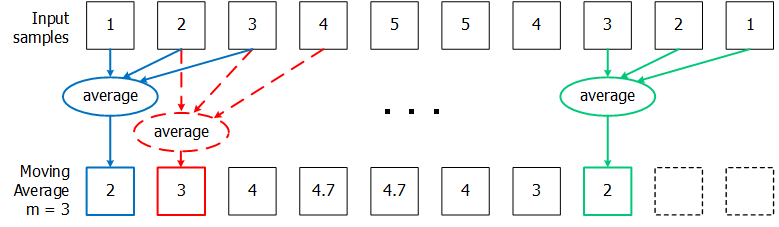
\includegraphics[scale=0.65]{Figures/MovAvg3.png}
\end{center}

\textbf{Example 2: Full moving average}

Ici, la séquence de sortie a la même taille que la séquence d'entrée.
Supposez que la dernière valeur d'entrée est répétée autant de fois que nécessaire.
Les valeurs des deux derniers échantillons de sortie (les deux manquants dans l'exemple précédent) sont alors $average(2,1,1) = 1.3$ et $average(1,1,1) = 1$, respectivement.
\begin{center}
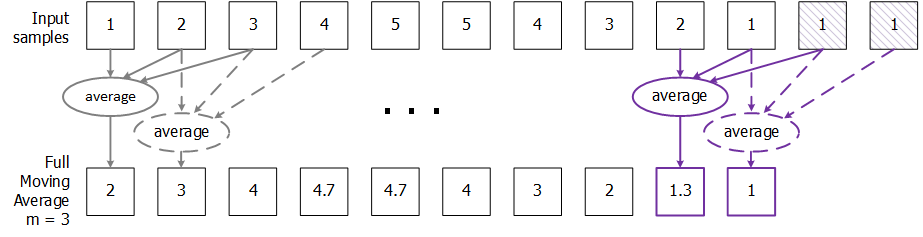
\includegraphics[scale=0.65]{Figures/FullMovAvg3.png}
\end{center}

Dans cet exercice, vous devez écrire un programme qui, pour une séquence d'entrées donnée, crée deux séquences de sortie: la première séquence est calculée avec la méthode du \textbf{simple moving average}, la deuxième avec celle du \textbf{full moving average}.
Suivez les instructions dans la page suivante.

\newpage
\begin{enumerate}[a)]

\item \textcolor{mygreen}{[Difficulté: **]}
Écrivez la fonction 

\begin{center}
\texttt{void movAvg(float *in, float *out, int m)}, 
\end{center}

qui prend comme arguments les adresses de début du tableau de données et du tableau contenant les moyennes, ainsi que la taille du groupe d'éléments utilisés pour calculer chaque moyenne. Cette fonction remplit le tableau des moyennes suivant le premier exemple (simple moving average) et affiche tous les éléments de ce tableau comme dans l'exemple de sortie au bas de cette page.

\item \textcolor{mygreen}{[Difficulté: ***]}
Écrivez la fonction

\begin{center} 
\texttt{void movAvgFull(float *in, float *out, int m)}, 
\end{center}

qui prend comme arguments les adresses de début du tableau de données et du tableau contenant les moyennes, ainsi que la taille du groupe d'éléments utilisés pour calculer chaque moyenne. Cette fonction remplit le tableau des moyennes suivant le deuxième exemple (full moving average) et affiche tous les éléments de ce tableau comme dans l'exemple de sortie au bas de cette page.

\vspace{20pt}
\hspace{-20pt} Continuez en écrivant tout ce qui manque pour compléter le programme, incluant ce qui suit :
\vspace{20pt}

\item \textcolor{mygreen}{[Difficulté: *]} Déclarez et initialisez un tableau de données de 10 éléments en virgule flottante dont les valeurs sont: 1, 2, 3, 4, 5, 5, 4, 3, 2 et 1.

\item \textcolor{mygreen}{[Difficulté: *]}  Votre programme doit être appelé avec un paramètre. Ce paramètre est le nombre d'éléments utilisés pour calculer les moyennes. (hint: il faut utiliser \texttt{argc/argv}, et pas \texttt{scanf}!)
	\begin{itemize}

	\item Si ce paramètre n'est pas spécifié ou plusieurs paramètres sont spécifiés, le programme doit afficher le message
	\begin{center}
	\textcolor{blue}{Incorrect number of program arguments.}
	\end{center}
	et ensuite terminer.

	\item Si la valeur de ce  paramètre est plus petite que 1 ou plus grande que la taille du tableau de données, le programme doit afficher le message
	\begin{center}
	\textcolor{blue}{Invalid program argument value.}
	\end{center}
	et ensuite terminer.

	\end{itemize}

\item \textcolor{mygreen}{[Difficulté: *]}  Le programme doit faire appel aux fonctions \texttt{movAvg} et \texttt{movAvgFull}.
\end{enumerate}

\vspace{20pt}

Exemple de sortie du programme pour \texttt{m = 3}:
\begin{center}
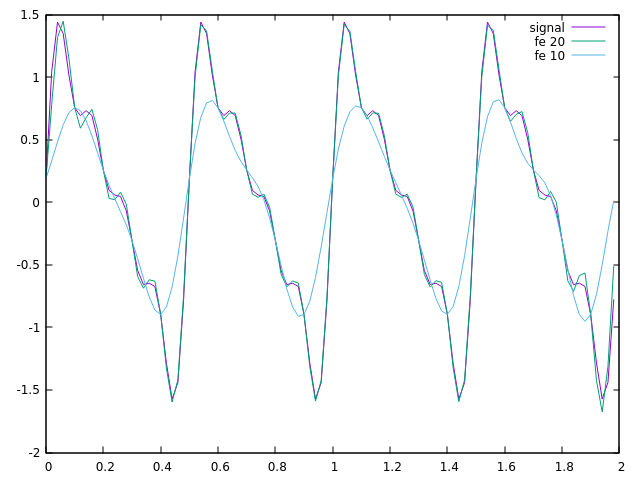
\includegraphics[scale=0.75]{Figures/Result.png}
\end{center}

\end{document}